\section{Introduction}

Integrity is doing the right thing even when no one is watching. - C.S. Lewis. Computational integrity (CI) refers to the assurance that a computation is well done executed and the results of that execution are accurate, reliable, and trustworthy. This document describes the assembly language created by Polygon, designed specifically with Ethereum Virtual Machine (EVM) features to represent blockchain transactional-based computations that could be executed with probable CI.


Ethereum is a decentralized, general-purpose blockchain computer where programs are represented as smart contracts and state transitions are triggered by users through the execution of transactions. One of the key components of Ethereum is the EVM. The EVM is a runtime environment that executes smart contracts on the Ethereum network. It provides a secure and isolated environment for executing code, and it ensures that the code is executed in a predictable and deterministic manner. 

When executing a transaction on the Ethereum network, a fee must be paid. The fee is proportional to the complexity of the computation and the demand on the network. The increasing demand for the Ethereum network, combined with its limited capacity, has caused the fees to rise to the point where they may impact the practical usability of the network. To address this issue, several layer 2 (L2) solutions have emerged in the market to improve the usability of Ethereum.

Polygon's zkEVM is a layer 2 network that implements a special instance of the Ethereum Virtual Machine (EVM). Although the network has a different architecture and state from Ethereum layer 1 (L1), communication with the Polygon zkEVM is done through a JSON-RPC interface that is fully compatible with Ethereum RPC, allowing all Ethereum-compatible applications and tools to be natively compatible with Polygon zkEVM. However, it's important to note that this is a separate instance with a distinct state from Ethereum L1, and as such, balances in accounts may not be the same and L1 smart contracts cannot be directly accessed through L2 transactions. Nevertheless, a bridge and cross-chain messaging mechanism enables the exchange of data between both networks (refer to the technical documents regarding the zkEVM bridge).



\subsection{Ethereum Virtual Machine Basics}

\subsection{Introduction}

The Ethereum blockchain is a digital ledger that keeps track of all transactions and interactions that occur on the Ethereum network.
Ethereum can store and execute smart contracts, which can perform a variety of tasks and operations on the network, 
in addition to recording transactions.
At any given time, a collection of data defines the current state of the Ethereum blockchain.
The Ethereum state includes account balances, smart contract code, smart contract storage and other information relevant to the operation of the network.
The Ethereum's state is maintained by each network node.

Some key features of the EVM:

\begin{itemize}
    \item \textbf{Deterministic}: This means it will always produce the same output given the same input.
    This feature is critical for ensuring the dependability and predictability of smart contract execution. 
    \item \textbf{Sandboxed}: This means that transactions processed by smart contracts run in an 
    environment that is isolated from the rest of the system, making it impossible for them to access or modify data outside this environment.
    This contributes to security by preventing unauthorized access to sensitive data. 
    \item \textbf{Stack-based}: This means that it employs a last-in first-out memory data structure for the basic processing of the operations, 
    with data being pushed onto a stack and popped off as needed. 
\end{itemize}

The EVM is made up of several key components that work together to execute smart contracts on the Ethereum blockchain
and provide the previous features.

\begin{figure}[H]
    \centering
    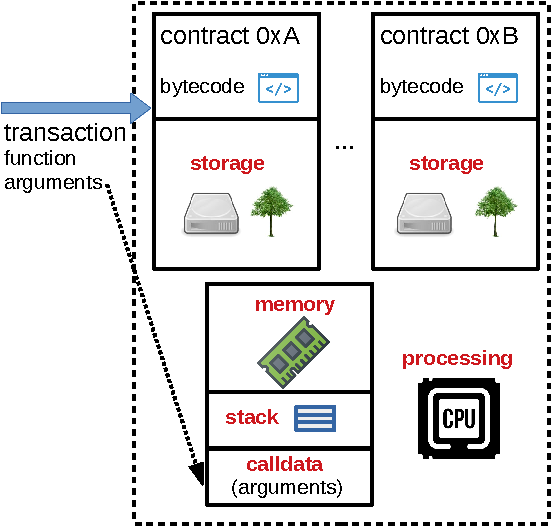
\includegraphics[width=.6\textwidth]{../figures/EVM-structure}
    \caption{EVM Components Involved in the Processing of a Transaction.}
    \label{fig:evm-transaction-processing}
\end{figure}

As shown in Figure \ref{fig:evm-transaction-processing}, the main components of the EVM involved in the processing of a transaction are the following:

\begin{itemize}
    \item \textbf{Smart Contract Bytecode}: This is the low-level code that is executed by the EVM.
    This bytecode is a series of opcodes, or machine-level instructions.
    Each opcode in the EVM bytecode corresponds to a specific operation, such as arithmetic, conditional branching, or memory manipulation.
    The EVM executes the bytecode in a step-by-step fashion, with each opcode being processed in sequence. 
    In general, smart contracts are written in a high-level programming language, such as Solidity, 
    and then compiled into EVM bytecode.
    \item \textbf{Processing Environment}: The processing environment is responsible for executing smart contracts. It provides a runtime environment for the contract bytecode to execute in and manages the memory and storage that the contract uses.
    \item \textbf{Stack}: The EVM is a stack-based machine, which means that it uses a stack data structure to execute its operations.
    \item \textbf{Memory}: The EVM also has a memory component that allows smart contracts to store and retrieve data. Memory is organized as a linear array of bytes, and data is accessed by specifying the memory location.
    \item \textbf{Calldata}: The transaction that invokes a smart contract contains a set of parameters and values required for the smart contract to perform its function.
    These parameters and values are passed to the smart contract as calldata.
    Calldata is read-only, which means that the smart contract cannot modify it during execution.
    This is due to the fact that the input data is part of the transaction that is stored on the blockchain, and any changes to the input data result in a different transaction hash and a different state of the blockchain. 
    \item \textbf{Storage}: Smart contracts can also store data in the EVM's storage component. Storage is a persistent key-value store that is associated with each contract and can be used to store state information.
\end{itemize}

The EVM is a variant of the von Neumann architecture that uses a single shared memory for both data and instructions.
The smart contract's bytecode is stored in memory in the EVM, and the program counter (PC) keeps track of the current instruction being executed.
The stack is used to hold values that are needed for immediate use, such as function parameters, local variables, and return values. The stack is typically used for storing small values, such as integers and booleans while, the memory is used for storing large data structures, such as arrays and strings.

On the other hand, the EVM has its own instruction set or list of available opcodes, which is a set of low-level commands that are used to manipulate data in the stack, memory, and storage components. The instruction set includes operations such as arithmetic, bit manipulation, and control flow.
In addition, to prevent spam and denial-of-service attacks, the EVM employs a gas system.
Gas is a unit of measurement for the computational resources required to execute a smart contract, and each operation in the instruction set has its own gas cost. 


\subsection{EVM Stack}

The EVM is a stack-based machine, which means that it uses a stack data structure to execute its operations.
When an operation is performed, it uses the values that are currently on the top of the stack, and then pushes the result back onto the stack.
Some of the main stack operations in the EVM are:

\begin{itemize}
    \item \texttt{PUSH}: Pushes a value onto the stack. The opcode is followed by a byte indicating the number of bytes to be pushed onto the stack, and the actual bytes to be pushed. For example, the opcode "PUSH2 0x0123" pushes the value 0x0123 onto the stack.
    \item \texttt{POP}: Removes the top value from the stack and discards it.
    \item \texttt{DUP}: Duplicates the top value on the stack and pushes the duplicate onto the stack.
    \item \texttt{SWAP}: Swaps the top two values on the stack.
    \item \texttt{ADD}, \texttt{SUB}, \texttt{MUL}, \texttt{DIV}, \texttt{MOD}: These opcodes perform arithmetic operations on the top two values of the stack, and push the result back onto the stack.
    \item \texttt{AND}, \texttt{OR}, \texttt{XOR}, \texttt{NOT}: These opcodes perform bitwise logic operations on the top two values of the stack, and push the result back onto the stack.
    \item \texttt{EQ}, \texttt{LT}, \texttt{GT}: These opcodes perform comparison operations on the top two values of the stack, and push the result back onto the stack as a boolean.
    \item \texttt{SHA3}: Computes the SHA3 hash of the top value on the stack, and pushes the hash onto the stack.
    \item \texttt{JUMP}, \texttt{JUMPI}: These opcodes modify the program counter, allowing the program to jump to a different part of the code.
\end{itemize}

The EVM stack is limited to 1024 elements.
If a contract attempts to push more elements onto the stack than this limit, a stack overflow error will occur, causing the transaction to fail. 

\subsection{EVM Memory}
The memory in the EVM is used for storing large data structures, such as arrays and strings.
This memory is a linear array of bytes that is used by smart contracts to store and retrieve data. 
The size of the memory is dynamically allocated at runtime, meaning that the amount of memory available to a smart contract can grow depending on its needs.
The EVM memory is byte-addressable, which means that each byte in the memory can be individually addressed using a unique index. The size of the words in the EVM is 256 bits (32 bytes), which means that data is typically loaded and stored in 32-byte chunks. The EVM also provides instructions for loading and storing smaller chunks of data, such as individual bytes or 16-bit words.
The EVM memory is non-persistent, which means that it is cleared whenever a smart contract execution completes. This means that if a contract wants to store data permanently, it must use the EVM storage component instead.
It's also worth noting that the use of memory in the EVM is subject to gas costs. This is because accessing and modifying memory requires computational resources, which are paid for in the form of gas.
The current memory limit for smart contracts on the Ethereum network is $2^{16}$ (or 65,536) pages. This means that the maximum amount of memory that a contract can use is 2 megabytes. 

When a contract calls another contract, a new execution environment is created with its own memory space.
The parent contract's memory space is saved, and the new contract's memory space is initialized.
The new contract can then make use of its memory as needed.
When the called contract's execution is complete, the memory space is released and the parent contract's saved memory is restored. 
It's worth noting that if a smart contract does not actually use the memory it has been allocated, that memory cannot be reclaimed or reused in the execution context of another contract.
The opcodes related to memory are the following:

\begin{itemize}
    \item \texttt{MLOAD}: This opcode is used to load a 32-byte word from memory into the stack. It takes a memory address as its input and pushes the value stored at that address onto the stack.
    \item \texttt{MSTORE}: This opcode is used to store a 32-byte word from the stack into memory. It takes a memory address and a value from the stack as its input, and stores the value at the specified address.
    \item \texttt{MSTORE8}: This opcode is similar to MSTORE, but it stores a single byte of data instead of a 32-byte word. It takes a memory address and a byte value from the stack as its input, and stores the byte at the specified address.
    \item \texttt{MSIZE}: This opcode returns the size of the current memory area in bytes.
\end{itemize}




\subsection{EVM Storage}

The EVM storage is a persistent key-value store that is associated with each smart contract. 
Storage is organized as a large array of 32-byte words and each word is identified by a unique 256-bit key, 
which is used to access and modify the value stored in that word.
Because the storage is non-volatile, data stored in it will persist even after the contract execution is completed. 
Accessing and modifying storage is a relatively expensive operation in terms of gas costs.
The EVM storage is implemented using a modified version of the Merkle Patricia Tree data structure, which allows for efficient access and modification of the storage data. 
A Patricia tree is a specific type of trie that is designed to be more space-efficient than a standard trie, by storing only the unique parts of the keys in the tree.
Patricia trees are particularly useful in scenarios where keys share common prefixes, as they allow for more efficient use of memory and faster lookups compared to standard tries.
The opcodes to manipulate the storage of a smart contract are the following:

\begin{itemize}
    \item \texttt{SLOAD}: This opcode loads a 256-bit word from storage at a given index and pushes it onto the stack.
    \item \texttt{SSTORE}: This opcode stores a 256-bit word to storage at a given index. The value to be stored is popped from the stack, and the index is specified as the next value on the stack.
\end{itemize}


\subsection{Transaction Processing}

An Ethereum transaction is processed by first decoding it to obtain relevant fields such as the recipient address, 
the amount of Ether being transferred, and the data payload.
To encode and decode transaction data, the RLP (Recursive Length Prefix) is used.
Transactions are digitally signed using ECDSA (Elliptic Curve Digital Signature Algorithm).
An important feature of ECDSA is that the signing public key can be recovered from the transaction signature
without requiring the user to explicitly provide it in the transaction.
The associated Ethereum account, which is identified by a 20-byte (160-bit) address, is then computed using the public key. 
The address is derived from the public key associated with the account by computing the Keccak-256 hash of the public key and
taking the last 20 bytes of this hash.

When processing a transaction, the EVM begins by creating a context with an empty stack and memory space.
The bytecode instructions are then executed, with values pushed and popped on the stack as needed. 
The EVM also uses a program counter to keep track of which instruction to execute next. 
Each opcode has a fixed number of bytes, so the program counter increments by the appropriate 
number of bytes after each instruction is executed.
The stack elements have a size of 32 bytes each. This means that each value pushed onto the stack by an opcode, as well as each value popped off the stack by an opcode, is 32 bytes in size.
The 32-byte size limit is a fundamental design choice in Ethereum and is based on the size of the EVM word. The EVM word is the basic unit of storage and processing in the EVM, and it is defined as a 256-bit (32-byte) unsigned integer.
Since the EVM word is the smallest unit of data that can be processed by the EVM, the stack elements are also designed to be 32 bytes in size.

To summarize, the EVM sequentially executes the opcodes in the bytecode, following the program counter, and manipulates 32-byte values on the stack and in memory as needed to perform the desired computations and store the desired values to persist.

\subsection{EVM interpreter}

EVM interpreter is a software component that can process and execute Ethereum transactions. 

Ethereum smart contracts can be written in various programming languages, such as Solidity, Vyper, Fe, or Yul, but are ultimately compiled into a sequence of EVM opcodes, expressed as bytecodes, that can be interpreted by the EVM interpreter. Ethereum opcodes are the low-level instruction set for EVM and represent the basic operations that EVM can perform during the execution of a smart contract triggered by a transaction.

The list of Ethereum op codes includes over 200 different operations , ranging from general arithmetic and logical operations to more advanced and blockchain eviroment specific operations like calls to other contracts, contract creation, and storage management. Some of the most commonly used op codes include:

\begin{itemize}
    \item \textbf{ADD, SUB, MUL, DIV:} Basic arithmetic operations.
    \item \textbf{CALL, DELEGATECALL, CALLCODE:} Calling other contracts.
    \item \textbf{PUSH, POP:} Stack management operations.
    \item \textbf{JUMP, JUMPI:} Conditional jumps for making decisions.
    \item \textbf{SLOAD, SSTORE:} Storage management operations.
    \item \textbf{MLOAD, MSTORE:} Memory management operations.
\end{itemize}

\subsection{zkASM and the ROM}
The zero-knowledge Assembly (zkASM) is an assembly language designed by Polygon to describe computations that can be executed by a "special" virtual machine. This virtual machine has the ability to not only compute an output from a computation description and a set of inputs, but also generate a succinct cryptographic CI proof of a fixed length. This proof can be verified using a fixed and, more importantly, a low amount of energy and time. To achieve this “special” behavior, this virtual machine relies on Zero Knowledge technology. 

Therefore, for any computation described in zkASM and executed with this "special" virtual machine its CI can be verified using fewer computational resources than were required for the original computation. The trick is that the proof verification algorithm can be implemented using a Ethereum smart contracts language and deployed on Ethereum L1, so for any computation expressed in zkASM its CI can be efficiently verified on Ethereum L1 using a fixed and low amount of gas, thereby inheriting Ethereum L1 security while avoiding network overhead. 

In Ethereum L1, transactions are grouped into blocks. Each block contains an ordered sequence of transactions that are executed in a deterministic manner over Ethereum state, resulting in a new version of the Ethereum L1 state. Unlike Ethereum L1, in Polygon's zkEVM, the data structure that contains an ordered set of transactions that represents a state transition, is called a batch.

The ROM is a zkASAM program that is an EVM interpreter for Polygon zkEVM's batches architecture, all EVM opcodes are implemented on it aswell the batch interpretation and transaction execution logic in such a way that by the use of the ROM, our "special" virtual machine, given an Polygon's zkEVM L2 State and a batch of transactions, can execute those transactions, compute the resulting L2 State and generate a CI proof of the state transition. In order to verify the CI proofs, and provide data availability to the batches data, a sophisticated protocol has been designed and deployed on Ethereum L1 (refer to the technical documents regarding the zkEVM state management). The advantage of this design is that it enables the creation of a highly efficient Ethereum network (Polygon zkEVM) on top of Ethereum L1, inheriting its security, moreover most of the Ethereum ecosistem will be natively compatible with this new network. ROM stands for Read-Only Memory, due to its analogy with computer memories. Indeed the system can be viewed as a silicon processor capable of interpreting a set of instructions and a ROM memory containing a firmware (a piece of low-level software that is infrequently subjected to changes) written with that set of instructions which implements a special EVM interpreter for Polygon zkEVM L2 architecture. To operate, the processor executes the ROM's program which takes as inputs a batch of L2 transactions to be executed and the previous L2 State, and produces a new state and a CI proof as output. The system composed of the zk "special" virtual machine and the ROM is called the zkEVM batch prover.

Figure 1 shows a high level overview of the zkEVM batch prover.

\begin{figure}[H]
    \centering
    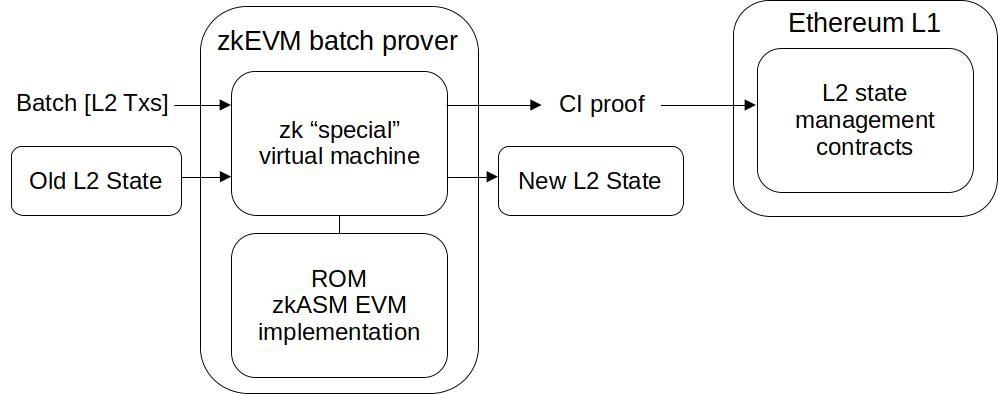
\includegraphics[width=0.8\columnwidth]{\assemblydir/figures/Introduction-schema}
    \caption{zkEVM batch prover structure.}
    \label{fig:hashk-add-bytes}
\end{figure}



In order to avoid futures misunderstood, it would be helpful to define and distinguish between the zkASM assembly instructions set and the EVM opcodes at this point.

\begin{itemize}
    \item \textbf{zkASM instructions:} Set of instructions created and developed by Polygon to target a "special" zero-knowledge virtual machine that can execute computations with probable CI.
    \item \textbf{EVM opcodes:} Set of instructions designed to target the EVM, used to define smart contract's computations.
\end{itemize}

Although zkASM instructions and EVM opcodes are different types of instructions, the Polygon zkEVM ROM contains a piece of code written in zkASM instructions to implement each EVM opcode.
